% Created 2015-05-07 jue 12:40
\documentclass[xcolor={usenames,svgnames,dvipsnames}]{beamer}
\usepackage[utf8]{inputenc}
\usepackage[T1]{fontenc}
\usepackage{fixltx2e}
\usepackage{graphicx}
\usepackage{longtable}
\usepackage{float}
\usepackage{wrapfig}
\usepackage{rotating}
\usepackage[normalem]{ulem}
\usepackage{amsmath}
\usepackage{textcomp}
\usepackage{marvosym}
\usepackage{wasysym}
\usepackage{amssymb}
\usepackage{hyperref}
\tolerance=1000
\usepackage{color}
\usepackage{listings}
\usecolortheme{rose}
\setbeamercolor{alerted text}{fg=Blue}
\setbeamerfont{alerted text}{series=\bfseries}
\setbeamercolor{block title}{bg=structure.fg!20!bg!50!bg}
\setbeamercolor{block body}{use=block title,bg=block title.bg}
\setbeamertemplate{navigation symbols}{}
\AtBeginSubsection[]{\begin{frame}[plain]\tableofcontents[currentsubsection,sectionstyle=show/shaded,subsectionstyle=show/shaded/hide]\end{frame}}
\lstset{keywordstyle=\color{blue}, commentstyle=\color{gray!90}, basicstyle=\ttfamily\small, columns=fullflexible, breaklines=true,linewidth=\textwidth, backgroundcolor=\color{gray!23}, basewidth={0.5em,0.4em}, literate={á}{{\'a}}1 {ñ}{{\~n}}1 {é}{{\'e}}1 {ó}{{\'o}}1 {º}{{\textordmasculine}}1}
\usepackage{mathpazo}
\hypersetup{colorlinks=true, linkcolor=Blue, urlcolor=Blue}
\usepackage{fancyvrb}
\DefineVerbatimEnvironment{verbatim}{Verbatim}{fontsize=\tiny, formatcom = {\color{black!70}}}
\usetheme{Goettingen}
\usefonttheme{serif}
\author{Oscar Perpiñán Lamigueiro \\ \url{http://oscarperpinan.github.io}}
\date{}
\title{Gráficos con R}
\hypersetup{
  pdfkeywords={},
  pdfsubject={},
  pdfcreator={Emacs 24.4.1 (Org mode 8.2.7c)}}
\begin{document}

\maketitle
\begin{frame}{Outline}
\tableofcontents
\end{frame}



\section{Introducción}
\label{sec-1}
\begin{frame}[fragile,label=sec-1-1]{Base y grid}
 \begin{itemize}
\item En \texttt{R} existen dos formas de generar gráficos:
\begin{itemize}
\item Base graphics
\item Grid graphics
\end{itemize}
\item Los gráficos base sólo producen un resultado gráfico, pero no un objeto.
\item Los gráficos \texttt{grid} generan un resultado gráfico \alert{y} un objeto.
\end{itemize}
\end{frame}

\begin{frame}[fragile,label=sec-1-2]{Gráficos \texttt{lattice}}
 Dentro del conjunto \texttt{grid} existen dos grandes paquetes:

\begin{block}{\texttt{lattice}}
\begin{itemize}
\item Implementación de los gráficos \emph{trellis}, \emph{The Elements of Graphing Data} de Cleveland)

\item Estructura matricial de paneles definida a través de una fórmula.
\end{itemize}

\lstset{language=R,label= ,caption= ,numbers=none}
\begin{lstlisting}
xyplot(wt ~ mpg | am, data = mtcars, groups = cyl)
\end{lstlisting}
\end{block}
\end{frame}

\begin{frame}[fragile,label=sec-1-3]{Gráficos \texttt{ggplot2}}
 Dentro del conjunto \texttt{grid} existen dos grandes paquetes:

\begin{block}{\texttt{ggplot2}}
\begin{itemize}
\item Implementación de \emph{The Grammar of Graphics} de Wilkinson.

\item Combinación de funciones que proporcionan los componentes (capas) del gráfico.
\end{itemize}

\lstset{language=R,label= ,caption= ,numbers=none}
\begin{lstlisting}
ggplot(mtcars, aes(mpg, wt)) +
    geom_point(aes(colour=factor(cyl))) +
    facet_grid(. ~ am)
\end{lstlisting}
\end{block}
\end{frame}

\section{Datos de ejemplo}
\label{sec-2}
\begin{frame}[fragile,label=sec-2-1]{Leemos desde el archivo local}
 \lstset{language=R,label= ,caption= ,numbers=none}
\begin{lstlisting}
  aranjuez <- read.csv('data/aranjuez.csv')

  summary(aranjuez)
\end{lstlisting}
\end{frame}

\begin{frame}[fragile,label=sec-2-2]{Añadimos algunas columnas}
 \lstset{language=R,label= ,caption= ,numbers=none}
\begin{lstlisting}
aranjuez$date <- as.Date(aranjuez$X)
\end{lstlisting}
\lstset{language=R,label= ,caption= ,numbers=none}
\begin{lstlisting}
  aranjuez$month <- as.numeric(
                    format(aranjuez$date, '%m'))

  aranjuez$year <- as.numeric(
                   format(aranjuez$date, '%Y'))

  aranjuez$day <- as.numeric(
                  format(aranjuez$date, '%j'))

  aranjuez$quarter <- quarters(aranjuez$date)
\end{lstlisting}
\end{frame}


\section{lattice}
\label{sec-3}

\begin{frame}[fragile,label=sec-3-1]{lattice}
 \begin{itemize}
\item Documentación: \href{http://lmdvr.r-forge.r-project.org/figures/figures.html}{Código y Figuras del libro}
\end{itemize}

\lstset{language=R,label= ,caption= ,numbers=none}
\begin{lstlisting}
  library(lattice)
\end{lstlisting}
\end{frame}

\begin{frame}[fragile,label=sec-3-2]{\texttt{xyplot}}
 \lstset{language=R,label= ,caption= ,numbers=none}
\begin{lstlisting}
  xyplot(Radiation ~ TempAvg, data=aranjuez)
\end{lstlisting}
\end{frame}

\begin{frame}[label=sec-3-3]{}
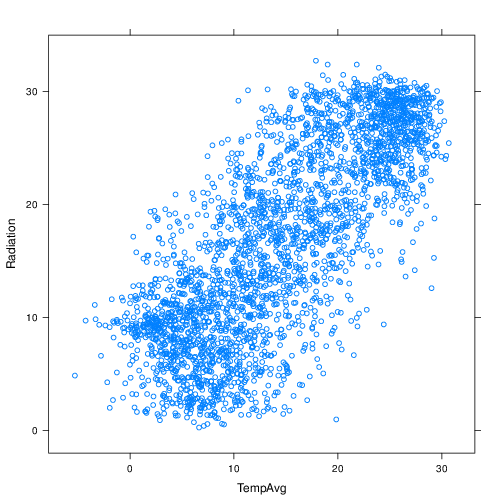
\includegraphics[width=.9\linewidth]{figs/xyplot.png}
\end{frame}


\begin{frame}[fragile,label=sec-3-4]{Añadimos rejilla}
 \lstset{language=R,label= ,caption= ,numbers=none}
\begin{lstlisting}
  xyplot(Radiation ~ TempAvg, data=aranjuez,
         grid = TRUE)
\end{lstlisting}
\end{frame}

\begin{frame}[label=sec-3-5]{}
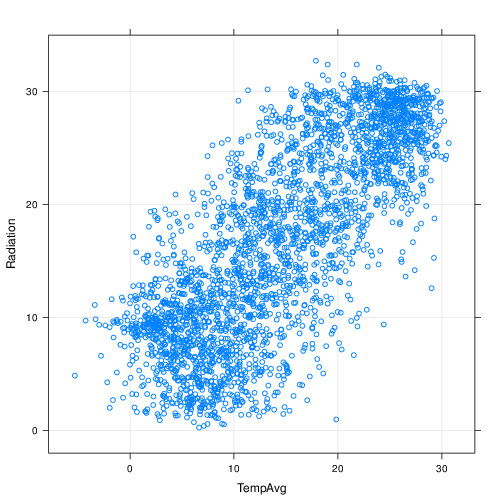
\includegraphics[width=.9\linewidth]{figs/xyplotPG.png}
\end{frame}


\begin{frame}[fragile,label=sec-3-6]{Añadimos regresión lineal}
 \lstset{language=R,label= ,caption= ,numbers=none}
\begin{lstlisting}
  xyplot(Radiation ~ TempAvg, data=aranjuez,
         type=c('p', 'r'), grid = TRUE,
         lwd=2, col.line='black')
\end{lstlisting}
\end{frame}

\begin{frame}[label=sec-3-7]{}
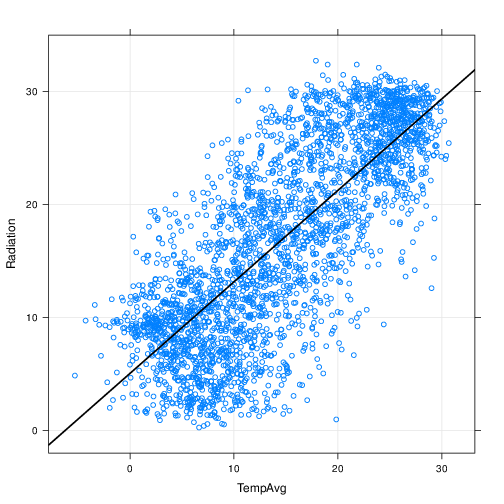
\includegraphics[width=.9\linewidth]{figs/xyplotPRG.png}
\end{frame}



\begin{frame}[fragile,label=sec-3-8]{Añadimos ajuste local}
 \lstset{language=R,label= ,caption= ,numbers=none}
\begin{lstlisting}
  xyplot(Radiation ~ TempAvg, data=aranjuez,
         type=c('p', 'smooth'), grid = TRUE,
         lwd=2, col.line='black')
\end{lstlisting}
\end{frame}

\begin{frame}[label=sec-3-9]{}
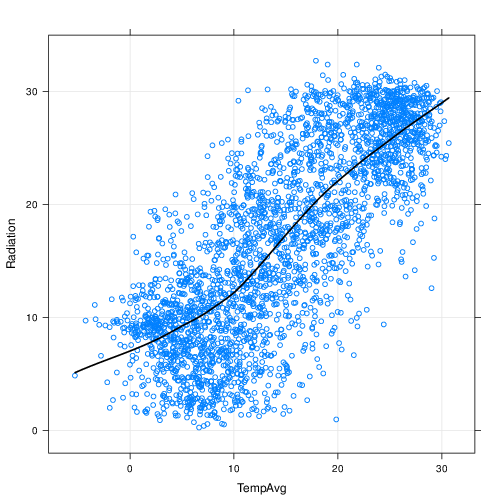
\includegraphics[width=.9\linewidth]{figs/xyplotSmooth.png}
\end{frame}


\begin{frame}[fragile,label=sec-3-10]{Paneles}
 \lstset{language=R,label= ,caption= ,numbers=none}
\begin{lstlisting}
  xyplot(Radiation ~ TempAvg|factor(year),
         data=aranjuez)
\end{lstlisting}
\end{frame}

\begin{frame}[label=sec-3-11]{}
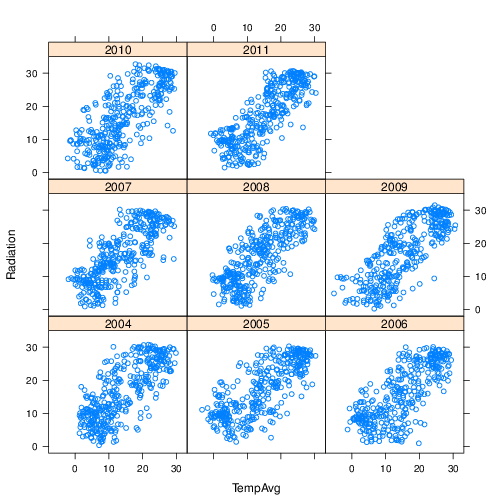
\includegraphics[width=.9\linewidth]{figs/xyplotYear.png}
\end{frame}

\begin{frame}[fragile,label=sec-3-12]{Grupos}
 \lstset{language=R,label= ,caption= ,numbers=none}
\begin{lstlisting}
  xyplot(Radiation ~ TempAvg, groups=quarter,
         data=aranjuez, auto.key=list(space='right'))
\end{lstlisting}
\end{frame}

\begin{frame}[label=sec-3-13]{}
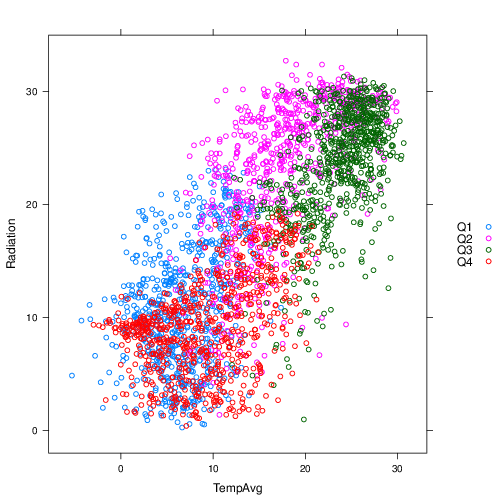
\includegraphics[width=.9\linewidth]{figs/xyplotQuarter.png}
\end{frame}

\begin{frame}[fragile,label=sec-3-14]{Paneles y grupos}
 \lstset{language=R,label= ,caption= ,numbers=none}
\begin{lstlisting}
  xyplot(Radiation ~ TempAvg|factor(year),
         groups=quarter,
         data=aranjuez,
         layout=c(4, 2),
         auto.key=list(space='right'))
\end{lstlisting}
\end{frame}

\begin{frame}[label=sec-3-15]{}
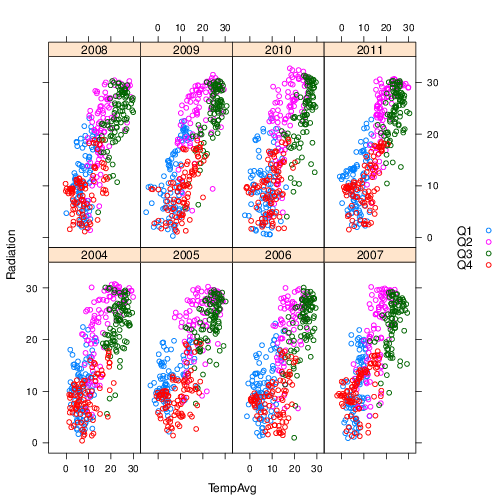
\includegraphics[width=.9\linewidth]{figs/xyplotQuarterYear.png}
\end{frame}

\begin{frame}[fragile,label=sec-3-16]{Paneles y grupos}
 \lstset{language=R,label= ,caption= ,numbers=none}
\begin{lstlisting}
  xyplot(Radiation ~ TempAvg|factor(year),
         groups=quarter,
         data=aranjuez,
         layout=c(4, 2),
         type=c('p', 'r'),
         auto.key=list(space='right'))
\end{lstlisting}
\end{frame}

\begin{frame}[label=sec-3-17]{}
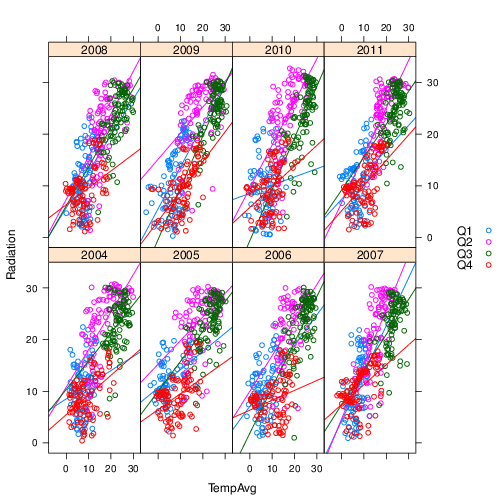
\includegraphics[width=.9\linewidth]{figs/xyplotQuarterYearSmooth.png}
\end{frame}

\begin{frame}[fragile,label=sec-3-18]{Colores y tamaños}
 \lstset{language=R,label= ,caption= ,numbers=none}
\begin{lstlisting}
  xyplot(Radiation ~ TempAvg,
         type=c('p', 'r'),
         cex=2, col='blue',
         alpha=.5, pch=19,
         lwd=3, col.line='black',
         data=aranjuez)
\end{lstlisting}
\end{frame}

\begin{frame}[label=sec-3-19]{}
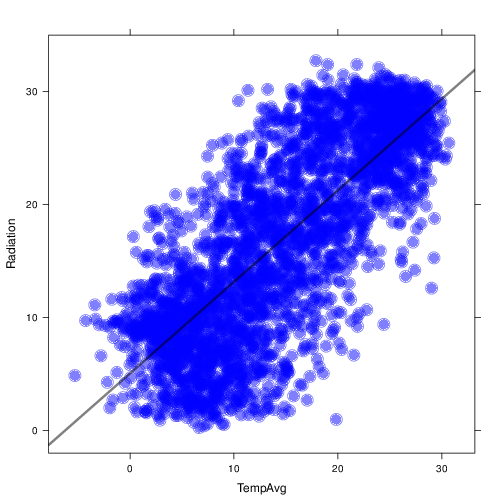
\includegraphics[width=.9\linewidth]{figs/xyplotColors.png}
\end{frame}

\begin{frame}[fragile,label=sec-3-20]{Colores con grupos}
 \lstset{language=R,label= ,caption= ,numbers=none}
\begin{lstlisting}
  xyplot(Radiation ~ TempAvg,
         group=quarter,
         col=c('red', 'blue', 'green', 'yellow'),
         pch=19,
         auto.key=list(space='right'),
         data=aranjuez)
\end{lstlisting}
\end{frame}

\begin{frame}[label=sec-3-21]{}
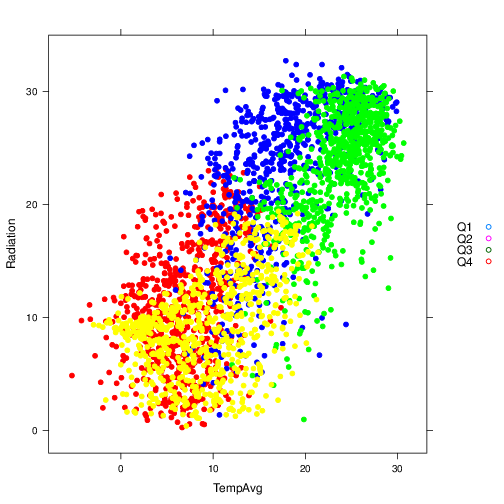
\includegraphics[width=.9\linewidth]{figs/xyplotColorGroups.png}
\end{frame}

\begin{frame}[fragile,label=sec-3-22]{Colores con grupos: \texttt{par.settings} y \texttt{simpleTheme}}
 \begin{itemize}
\item Primero definimos el tema con \texttt{simpleTheme}
\end{itemize}
\lstset{language=R,label= ,caption= ,numbers=none}
\begin{lstlisting}
  myTheme <- simpleTheme(col=c('red', 'blue',
                          'green', 'yellow'),
                          pch=19, alpha=.6)
\end{lstlisting}
\end{frame}

\begin{frame}[fragile,label=sec-3-23]{Colores con grupos: \texttt{par.settings} y \texttt{simpleTheme}}
 \begin{itemize}
\item Aplicamos el resultado en \texttt{par.settings}
\end{itemize}
\lstset{language=R,label= ,caption= ,numbers=none}
\begin{lstlisting}
  xyplot(Radiation ~ TempAvg,
         groups=quarter,
         par.settings=myTheme,
         auto.key=list(space='right'),
         data=aranjuez)
\end{lstlisting}
\end{frame}

\begin{frame}[label=sec-3-24]{}
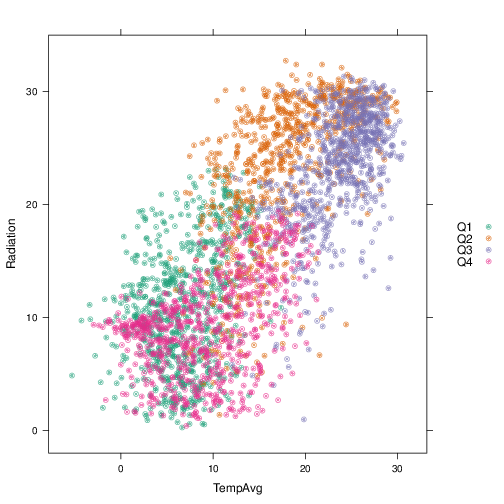
\includegraphics[width=.9\linewidth]{figs/myTheme.png}
\end{frame}

\begin{frame}[fragile,label=sec-3-25]{Colores: brewer.pal}
 \lstset{language=R,label= ,caption= ,numbers=none}
\begin{lstlisting}
library(RColorBrewer)

myPal <- brewer.pal(n = 4, 'Dark2')

myTheme <- simpleTheme(col = myPal,
                       pch=19, alpha=.6)
\end{lstlisting}

\begin{block}{ColorBrewer: \url{http://colorbrewer2.org/}}
\end{block}
\end{frame}

\begin{frame}[fragile,label=sec-3-26]{Asignamos paleta con \texttt{par.settings}}
 \lstset{language=R,label= ,caption= ,numbers=none}
\begin{lstlisting}
xyplot(Radiation ~ TempAvg,
       groups=quarter,
       par.settings=myTheme,
       auto.key=list(space='right'),
       data=aranjuez)
\end{lstlisting}
\end{frame}

\begin{frame}[label=sec-3-27]{}
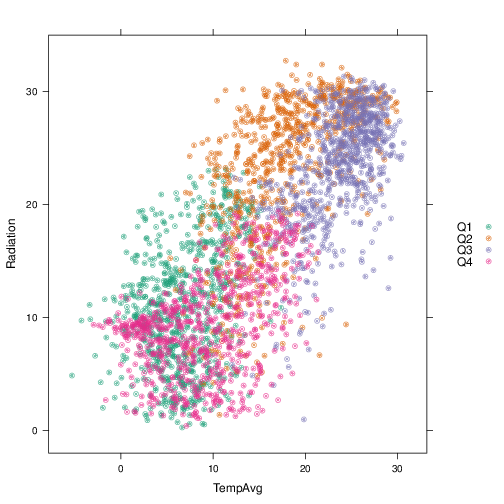
\includegraphics[width=.9\linewidth]{figs/brewer.png}
\end{frame}

\begin{frame}[fragile,label=sec-3-28]{Paneles a medida}
 \lstset{language=R,label= ,caption= ,numbers=none}
\begin{lstlisting}
  xyplot(Radiation ~ TempAvg, data=aranjuez,
         panel=function(x, y, ...){
             panel.xyplot(x, y, ...)
             minIdx <- which.min(x)
             maxIdx <- which.max(x)
             panel.points(x[c(minIdx, maxIdx)],
                          y[c(minIdx, maxIdx)],
                          cex=2, col='red')
             panel.text(x[minIdx], y[minIdx],
                        'MIN', pos=1)
             })
\end{lstlisting}
\end{frame}

\begin{frame}[label=sec-3-29]{}
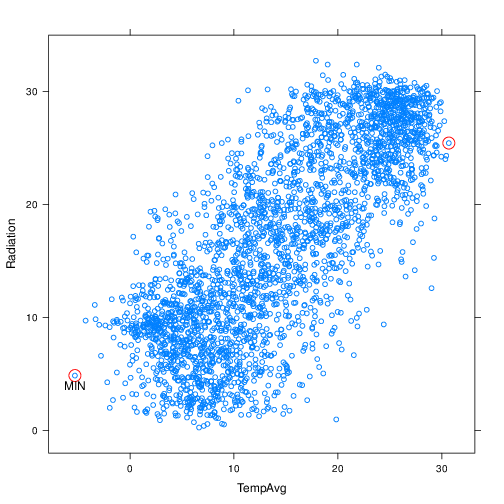
\includegraphics[width=.9\linewidth]{figs/panel.png}
\end{frame}

\begin{frame}[fragile,label=sec-3-30]{Matriz de gráficos de dispersión}
 \lstset{language=R,label= ,caption= ,numbers=none}
\begin{lstlisting}
  splom(aranjuez[,c("TempAvg", "HumidAvg", "WindAvg",
                    "Rain", "Radiation", "ET")],
        pscale=0, alpha=0.6, cex=0.3, pch=19)
\end{lstlisting}
\end{frame}

\begin{frame}[label=sec-3-31]{}
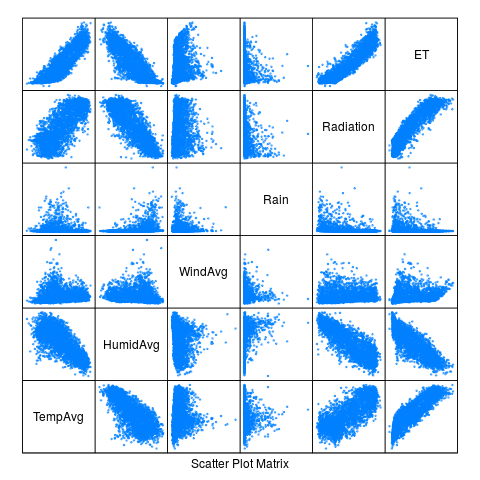
\includegraphics[width=.9\linewidth]{figs/splom.png}
\end{frame}

\begin{frame}[fragile,label=sec-3-32]{Matriz de gráficos de dispersión}
 \lstset{language=R,label= ,caption= ,numbers=none}
\begin{lstlisting}
  splom(aranjuez[,c("TempAvg", "HumidAvg", "WindAvg",
                    "Rain", "Radiation", "ET")],
        groups=aranjuez$quarter,
        auto.key=list(space='right'),
        pscale=0, alpha=0.6, cex=0.3, pch=19)
\end{lstlisting}
\end{frame}

\begin{frame}[label=sec-3-33]{}
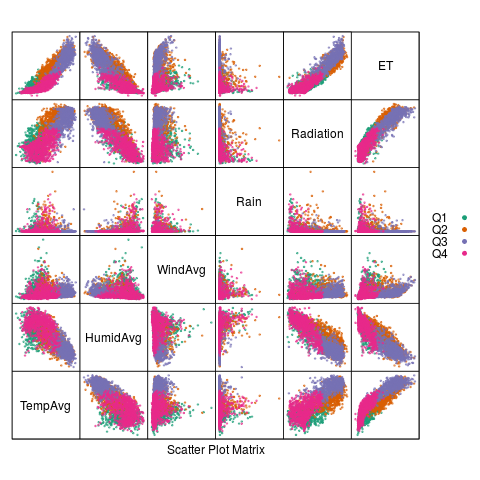
\includegraphics[width=.9\linewidth]{figs/splomGroup.png}
\end{frame}

\begin{frame}[fragile,label=sec-3-34]{\texttt{levelplot}}
 \lstset{language=R,label= ,caption= ,numbers=none}
\begin{lstlisting}
  levelplot(TempAvg ~ year * day, data = aranjuez)
\end{lstlisting}
\end{frame}

\begin{frame}[label=sec-3-35]{}
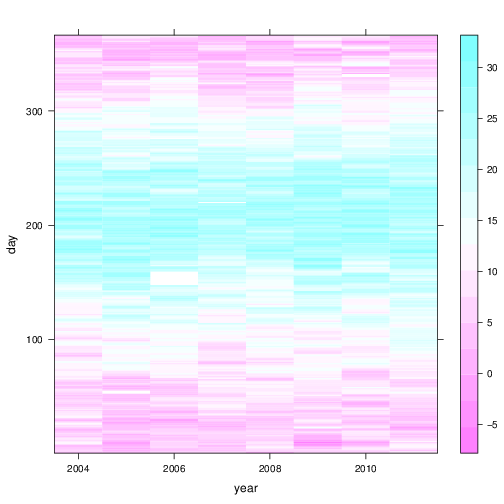
\includegraphics[width=.9\linewidth]{figs/levelplot.png}
\end{frame}

\begin{frame}[fragile,label=sec-3-36]{\texttt{levelplot} con una paleta mejor}
 \begin{itemize}
\item Usamos \texttt{colorRampPalette} para generar una función que interpola colores a partir de una paleta
\end{itemize}
\lstset{language=R,label= ,caption= ,numbers=none}
\begin{lstlisting}
levelPal <- colorRampPalette(
    brewer.pal(n = 9, 'Oranges'))
\end{lstlisting}
\begin{itemize}
\item Comprobamos que es una función generadora de colores
\end{itemize}

\lstset{language=R,label= ,caption= ,numbers=none}
\begin{lstlisting}
levelPal(14)
\end{lstlisting}

\begin{verbatim}
[1] "#FFF5EB" "#FEEBD9" "#FDE0C3" "#FDD3A8" "#FDC088" "#FDAB67" "#FD974A"
[8] "#F9812F" "#F16B16" "#E45709" "#D14501" "#B13A02" "#973003" "#7F2704"
\end{verbatim}

\begin{itemize}
\item Usamos esta función con \texttt{col.regions}
\end{itemize}
\lstset{language=R,label= ,caption= ,numbers=none}
\begin{lstlisting}
  levelplot(TempAvg ~ year * day,
            col.regions = levelPal,
            data = aranjuez)
\end{lstlisting}
\end{frame}

\begin{frame}[label=sec-3-37]{}
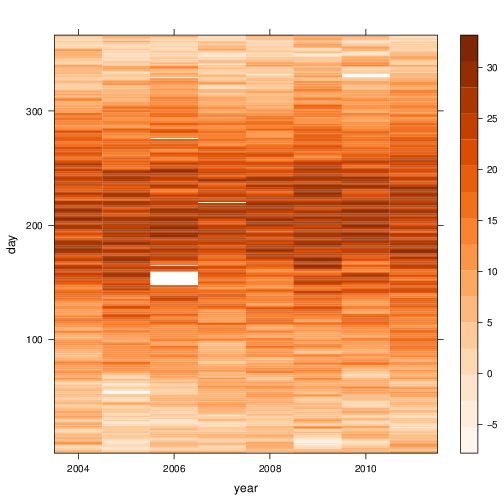
\includegraphics[width=.9\linewidth]{figs/levelplotPal.png}
\end{frame}

\begin{frame}[fragile,label=sec-3-38]{\texttt{contourplot}}
 \lstset{language=R,label= ,caption= ,numbers=none}
\begin{lstlisting}
  contourplot(TempAvg ~ year * day,
              data = aranjuez,
              lwd = .5,
              labels = list(cex = 0.6),
              label.style = 'align',
              cuts = 5)
\end{lstlisting}
\end{frame}

\begin{frame}[label=sec-3-39]{}
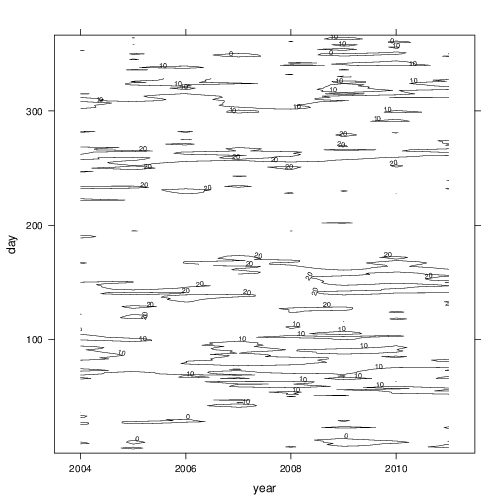
\includegraphics[width=.9\linewidth]{figs/contourplot.png}
\end{frame}

\begin{frame}[fragile,label=sec-3-40]{Box-and-Whiskers}
 \lstset{language=R,label= ,caption= ,numbers=none}
\begin{lstlisting}
  bwplot(Radiation ~ month, data=aranjuez,
         horizontal=FALSE, pch='|')
\end{lstlisting}
\end{frame}

\begin{frame}[label=sec-3-41]{}
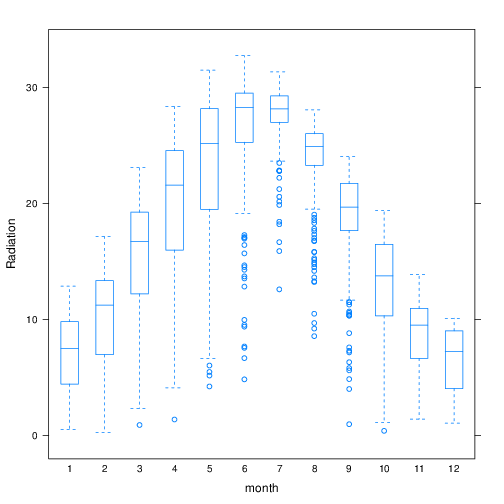
\includegraphics[width=.9\linewidth]{figs/bwplot.png}
\end{frame}

\begin{frame}[fragile,label=sec-3-42]{Box-and-Whiskers}
 \lstset{language=R,label= ,caption= ,numbers=none}
\begin{lstlisting}
  bwplot(Radiation ~ month, data=aranjuez,
         horizontal=FALSE,
         panel=panel.violin)
\end{lstlisting}
\end{frame}

\begin{frame}[label=sec-3-43]{}
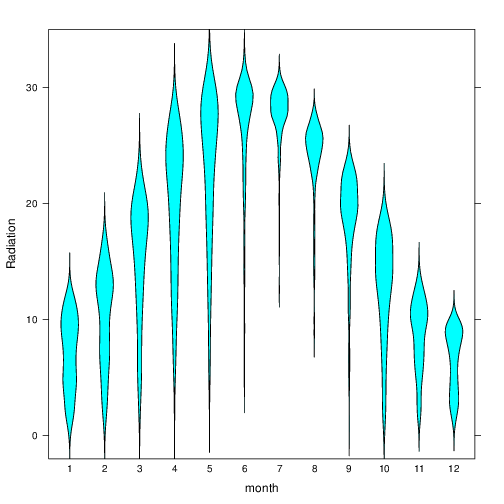
\includegraphics[width=.9\linewidth]{figs/violin.png}
\end{frame}


\begin{frame}[fragile,label=sec-3-44]{Histogramas}
 \lstset{language=R,label= ,caption= ,numbers=none}
\begin{lstlisting}
  histogram(~ Radiation|factor(year), data=aranjuez)
\end{lstlisting}
\end{frame}

\begin{frame}[label=sec-3-45]{}
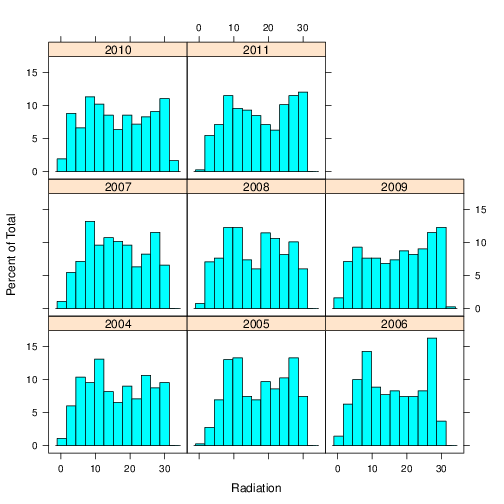
\includegraphics[width=.9\linewidth]{figs/histogram.png}
\end{frame}

\begin{frame}[fragile,label=sec-3-46]{Gráficos de densidad}
 \lstset{language=R,label= ,caption= ,numbers=none}
\begin{lstlisting}
densityplot(~ Radiation, groups=quarter,
            data=aranjuez,
            auto.key=list(space='right'))
\end{lstlisting}
\end{frame}

\begin{frame}[label=sec-3-47]{}
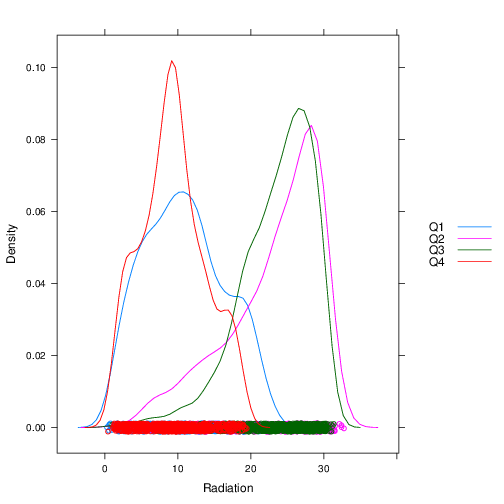
\includegraphics[width=.9\linewidth]{figs/density.png}
\end{frame}

\begin{frame}[fragile,label=sec-3-48]{\texttt{dotplot}}
 \lstset{language=R,label= ,caption= ,numbers=none}
\begin{lstlisting}
  avRad <- aggregate(Radiation ~ month * year,
                     data=aranjuez, FUN=mean)
\end{lstlisting}

\lstset{language=R,label= ,caption= ,numbers=none}
\begin{lstlisting}
  dotplot(month ~ Radiation|factor(year), data=avRad)
\end{lstlisting}
\end{frame}

\begin{frame}[label=sec-3-49]{}
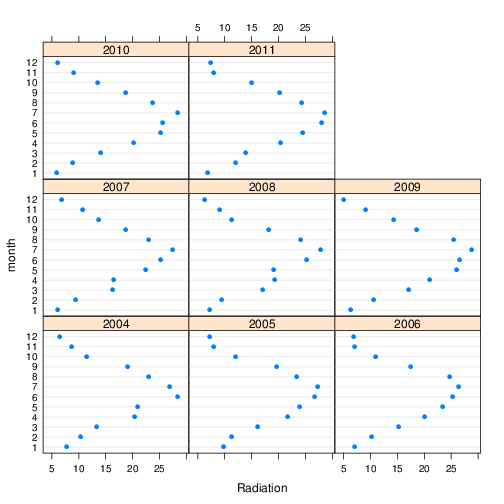
\includegraphics[width=.9\linewidth]{figs/dotplot.png}
\end{frame}


\begin{frame}[fragile,label=sec-3-50]{Quantile-Quantile}
 \lstset{language=R,label= ,caption= ,numbers=none}
\begin{lstlisting}
  firstHalf <- aranjuez$quarter %in% c('Q1', 'Q2')
  
  qq(firstHalf ~ Radiation, data=aranjuez)
\end{lstlisting}
\end{frame}

\begin{frame}[label=sec-3-51]{}
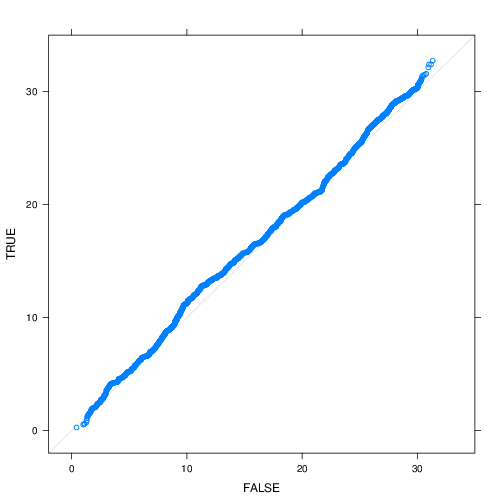
\includegraphics[width=.9\linewidth]{figs/qqHalf.png}
\end{frame}

\begin{frame}[fragile,label=sec-3-52]{Quantile-quantile}
 \lstset{language=R,label= ,caption= ,numbers=none}
\begin{lstlisting}
  winter <- aranjuez$quarter %in% c('Q1', 'Q4')
  
  qq(winter ~ Radiation, data=aranjuez)
\end{lstlisting}
\end{frame}

\begin{frame}[label=sec-3-53]{}
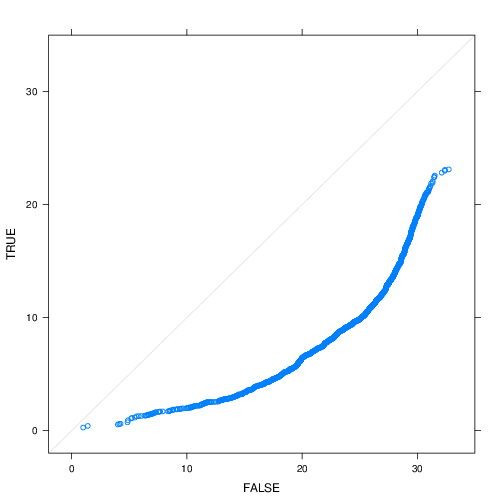
\includegraphics[width=.9\linewidth]{figs/qqWinter.png}
\end{frame}

\begin{frame}[fragile,label=sec-3-54]{Quantile-Quantile}
 \lstset{language=R,label= ,caption= ,numbers=none}
\begin{lstlisting}
  qqmath(~TempAvg, data=aranjuez,
         groups=year, distribution=qnorm)
\end{lstlisting}
\end{frame}

\begin{frame}[label=sec-3-55]{}
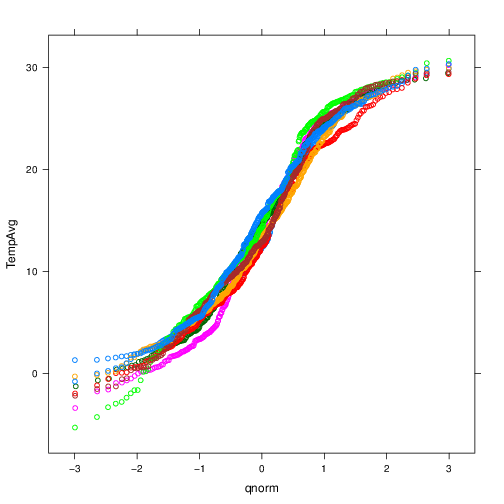
\includegraphics[width=.9\linewidth]{figs/qqNorm.png}
\end{frame}


\section{ggplot2}
\label{sec-4}
\begin{frame}[label=sec-4-1]{ggplot2}
\begin{itemize}
\item \href{http://docs.ggplot2.org/current/}{Documentación de ggplot2}
\item \href{http://ggplot2.org/book/}{Codigo del libro}
\item \href{http://learnr.wordpress.com/2009/06/28/ggplot2-version-of-figures-in-lattice-multivariate-data-visualization-with-r-part-1/}{ggplot2 desde lattice} (\href{http://learnr.files.wordpress.com/2009/08/latbook.pdf}{PDF})
\end{itemize}
\end{frame}
% Emacs 24.4.1 (Org mode 8.2.7c)
\end{document}